\section{BEHAVIORAL PATTERNS}
\subsection{Strategy}
Strategy pattern permit the definitions of many algorithms which served the same purpose. In this case, we used strategy patterns to define the way of calculating the price of the reservations. As mentioned in the previous section, we have implemented four decorators, two for flight reservation, two for hotel reservation. There're also four strategy classes corresponding to the decorators.

\begin{figure}[h]
\centering
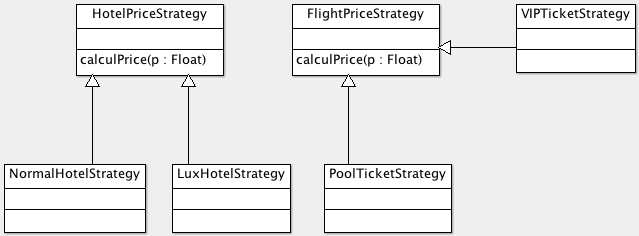
\includegraphics[width=12cm]{project/images/strategy.png}
\caption{Class diagram of strategies}
\end{figure}

\paragraph{}
Take an example of flight reservation's price's calculation. The method \textit{calculPrice} from two strategies are
\begin{lstlisting}
public class CheapHotelStrategy implements HotelPriceStrategy {
...
	@Override
	public float calculPrice(float p) {
		// TODO Auto-generated method stub
		return p * 80f / 100f;
	}
...
}

public class LuxHotelStrategy implements HotelPriceStrategy {
...
	@Override
	public float calculPrice(float p) {
		// TODO Auto-generated method stub
		return p * 120f / 100f;
	}
...
}
\end{lstlisting}

\subsection{Observer}
Observer pattern allow the objects, called observers, to be notified when there's a state change in the objects that were observed. In the context of this project, two observer classes were implemented to observe the number of available place in a flight and the number of free rooms in an hotel. Whenever these numbers reach zero, means that there are no more available space, the observers will display a message to notify the agent. 

\begin{figure}[h]
\centering
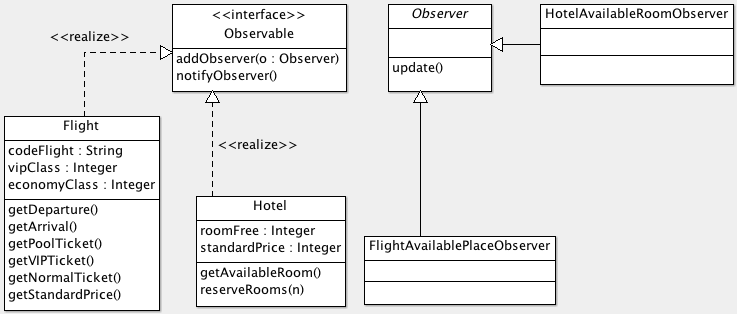
\includegraphics[width=12cm]{project/images/observer.png}
\caption{Class diagram of strategies}
\end{figure}

To implement this pattern, interface \textit{Observable} and abstract class \textit{Observer} are created. The classes that need to be observed will implement \textit{Observable}. After that, they should decide when to notify the observers. Take an example of class \textit{Flight}, in the code below we demonstrate the situation when the VIP's place is running out

\begin{lstlisting}
public void secureVIPPlace() {
	if (vipTickets >= 1) {
		vipTickets--;
		if (vipTickets == 0) {
			notifyObservers(FlightTicketType.VIP);
		}
	}
}
\end{lstlisting}

\newpage
\subsection{Iterator}
Iterator pattern allow the definition of an object, call \textit{iterator}, which can traverse the element objects of a container. There are two composite classes which could consider as a container: \textit{Client} and \textit{TravelTouringService}. We choose \textit{TravelTouringService} to deploy the iterator pattern. 

\begin{figure}[h]
\centering
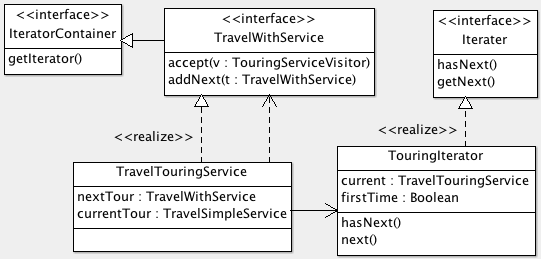
\includegraphics[width=12cm]{project/images/iterator.png}
\caption{Class diagram of iterator pattern}
\end{figure}

I implemented \textit{TouringIterator} as the inner class of \textit{TravelTouringService}. With this arrangement, \textit{TouringIterator} could freely access to \textit{nextTour}, an attribute that was caching by \textit{TravelTouringService}. \textit{TouringIterator} will return \textit{currentTour} and process to \textit{nextTour} each times the method \textit{getNext} is called. 

\begin{lstlisting}
public Object getNext() {
	if (hasNext()) {
		if (firstTime) {
			iter = current;
			firstTime = false;
		} else {
			iter = (TravelTouringService) iter.nextTour;
		}
		return iter.firstTour;
	}
	return null;
}
\end{lstlisting}

\newpage
\subsection{Visitor}



\subsection{Template}